\chapter{Progetto 2: Compressione di immagini tramite la DCT}

\section{Introduzione}
In questo progetto è stata implementata l'equazione della discrete cosine transform $2$ (DCT2).
La sua implementazione è stata realizzata applicando sequenzialmente sulla matrice
la discrete cosine transform $1$ (DCT) per righe e poi per colonne. In questo modo
è stato possibile riutilizzare più efficacemente il codice senza introdurre code
smells.

L'intero progetto è stato sviluppato in Julia, un linguaggio di programmazione ad
alto livello usato per il calcolo scientifico con tempi di esecuzione comparabili
con C/C++.

La libreria della FFT di Julia utilizzata è \href{https://github.com/JuliaMath/FFTW.jl}{FTTW}
che implementa un binding con la libreria di C, entrambe le librerie sono open source.

\section{DCT2 custom}
Come preannunciato in precedenza, è stato necessario concentrarsi solo in una implementazione
efficiente della DCT, la sua formula è stata riportata nell'equazione \ref{eq:dct}.

\begin{equation}
    X_k = \begin{cases}
        \sqrt{\frac{1}{N}}\cdot \sum_{n=0}^{N-1} x_n \cos\left[\frac{\pi}{N}\left(n + \frac{1}{2}\right) n \right] & k=1     \\
        \sqrt{\frac{2}{N}}\cdot\sum _{n=0}^{N-1}x_{n}\cos \left[\frac{\pi}{N}\left(n+\frac{1}{2}\right)n\right]    & k \ne 1
    \end{cases}
    \label{eq:dct}
\end{equation}

Per prima cosa è stato pensato di utilizzare un approccio basato su operazioni
tra vettori e matrice, più precisamente è stato pensato di pre-calcolare la matrice
della base dei coseni, per righe, prima di effettuare il calcolo dei coefficienti.
Successivamente si effettua un prodotto vettore-matrice per ottenere il vettore
dei coefficienti, infine si applica la normalizzazione su di essi.

Dato un generico vettore $X_k$, per applicare la dct si effettua:
\begin{equation*}
    dct(X_k) = norm(B_{\cos}\cdot X_k )
\end{equation*}

Dove $\cdot$ è il prodotto vettore matrice e $B_{\cos}$ è la base dei coseni creata
per riga, mentre $X_k$ è il vettore colonna iniziale. La funzione di normalizzazione
normalizza i coefficienti del vettore risultante nel seguente modo, normalizza
per $\sqrt{\frac{1}{N}}$ il primo coefficiente, mentre gli altri li normalizza
per $\sqrt{\frac{2}{N}}$.

L'implementazione della DCT2 si articola nel seguente modo:
\begin{itemize}
    \item si genera la base dei coseni per riga
    \item si applica inplace la DCT1 per righe
    \item si applica inplace la DCT1 per colonne
\end{itemize}

In questo modo si riescono ad ottenere dei tempi comparabili alla DCT2 implementata
dalla libreria usando la FFT.

\subsection{Studio di complessità}
L'algoritmo custom che è stato sviluppato ha dei tempi di esecuzione comparabili
con la libreria.

La complessità della DCT2 custom è la seguente:
\begin{itemize}
    \item \textbf{generazione della base dei coseni}: la generazione richiede
          un numero costante di operazioni tra scalari e un calcolo del coseno per ogni
          entry della matrice. Questo richiede un totale $\mathcal{O}(N^2)$ per generare
          la matrice, quando $N\times N$ è la dimensione della matrice (dimensione dello
          spazio vettoriale per numero di coefficienti).
    \item \textbf{applicazione della DCT1 su un vettore}: l'applicazione della DCT1
          su un generico vettore richiede di effettuare un prodotto matrice-vettore e
          successivamente di normalizzare i coefficienti. Il prodotto matrice-vettore
          ha una complessità asintotica di $\mathcal{O}(N^2)$, dove $N$ è la dimensione
          del vettore. Mentre per normalizzare i coefficienti si richiede una scansione
          lineare del vettore che richiede $\mathcal{O}(N)$, dove $N$ è la dimensione
          del vettore. Quindi complessivamente si ha una complessità di $\mathcal{O}(N^2 + N) = \mathcal{O}(N^2)$.
    \item \textbf{applicazione della DCT2 sull'intera matrice}: l'applicazione della DCT2
          sull'intera matrice richiede di eseguire una DCT1 per ogni riga e poi per ogni
          colonna. All'atto pratico non si rigenera ogni volta la matrice dei coseni,
          bensì inizialmente la si pre-calcola ($\mathcal{O}(N^2)$), successivamente si
          esegue la DCT1 per righe che richiede $\mathcal{O}(N \cdot N^2)$ ($N$ righe
          per $N^2$ la moltiplicazione riga-matrice) e successivamente si applica la
          DCT1 per colonne che richiede $\mathcal{O}(N \cdot N^2)$ ($N$ colonne
          per $N^2$ la moltiplicazione riga-matrice). Complessivamente si ottiene
          un $\mathcal{O}(N^3)$ a livello asintotico.
\end{itemize}

L'implementazione custom della DCT2 è stata confronta anche con quella ottimizzata
dalla libreria usando la FFT e nell'immagine \ref{fig:analisi_complex} si
può vedere il confronto.

\begin{figure}[!h]
    \centering
    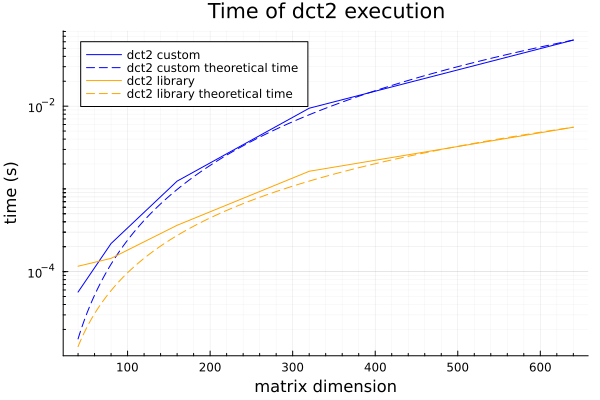
\includegraphics[width=0.5\textwidth]{Progetto_2/img/times_plot.png}
    \caption{Grafico dei tempi al variare della dimensione della matrice. Le linee
        continue rappresentano i dati empirici, le linee tratteggiate rappresentano
        l'andamento teorico dei metodi.}
    \label{fig:analisi_complex}
\end{figure}

Come si può notare dal grafico, l'andamento empirico segue quello teorico.

\section{Compressione}
In questa parte di progetto è stato implementata un'interfaccia web per ottenere
l'immagine bmp in scala di grigi

\subsection{Implementazione dell'interfaccia}

\subsection{Implementazione della compressione}
Dopo l'implementazione della GUI che si occupa di prendere in input l'immagine e
i due parametri, è stato sviluppato l'algoritmo di compressione dell'immagine.

L'implementazione della compressione si è articolata nel seguente modo:
\begin{itemize}
    \item \textbf{ridimensione dell'immagine in input}: l'immagine è stata ridimensionata
          in modo tale da avere altezza e larghezza multiple del parametro $f$.
    \item \textbf{implementazione della compressione}: la compressione è stata implementata
          applicando sui sotto-quadrati $f\times f$ dell'immagine la DCT2 della libreria,
          successivamente sono state azzerate le entry $k,l$ tali che $k+l\ge d$, infine
          si applica IDCT2 della libreria e si normalizzano i valori.
    \item \textbf{visualizzazione output}: infine vinee visualizzato l'output
          messo a confronto con l'input.
\end{itemize}

Nel dettaglio, la \textbf{ridimensione dell'immagine in input} elimina le ultime
righe e le ultime colonne dell'immagine in input in modo da avere le dimensioni
multiple di $f$.

Mentre, l'\textbf{implementazione della compressione} si articola nell'allocazione
di una matrice di appoggio $C\in \mathcal{R}^{f\times f}$ che viene inizializzata
su una sotto matrice $f\times f$ dell'immagine che si vuole elaborare.